
\حصہ{تکونیاتی تفاعل}
اس حصہ میں ریڈیئن، تکونی تفاعل، دوریت اور بنیادی تکونی مماثل پر غور کیا جائے گا۔ 

\جزوحصہء{ریڈیئن}
چھوٹی جماعتوں میں زاویوں کو درجات کی صورت میں ناپا جاتا ہے۔ احصاء میں زاویہ کو ریڈیئن میں ناپا جاتا ہے جہاں \عددی{180^{\circ}} کو \عددی{\pi} ریڈیئن کہتے ہیں۔ریڈیئن کی استعمال سے حساب آسان ہو جاتا ہے۔

فرض کریں \اصطلاح{اکائی دائرہ}\فرہنگ{اکائی!دائرہ}\حاشیہب{unit circle}\فرہنگ{unit!circle} (رداس \عددی{1} کا دائرہ) کا وسطی زاویہ \عددی{ACB} ہے (شکل \حوالہ{شکل_ابتدا_اکائی_دائرہ_ریڈیئن})۔زاویہ \عددی{ACB} کی ریڈیئن ناپ کی تعریف \ترچھا{اکائی دائرے} کی قوس \عددی{AB} کی لمبائی ہے۔چونکہ اکائی دائرے کا محیط \عددی{2\pi}  ہے اور ایک مکمل چکر \عددی{360^{\circ}} ہے لہٰذا درج ذیل تعلق لکھا جا سکتا ہے۔
\begin{align*}
\boxed{\pi\,\text{ریڈیئن}=180^{\circ}}
\end{align*}
%
\begin{figure}
\centering
\begin{tikzpicture}
\draw(0,0) circle (1);
\draw(0,0)node[below]{$C$}--++(10:1.2)node[shift={(-80:0.2)}]{$A$}node[pos=0.5,shift={(-80:0.2)}]{$1$};
\draw(0,0)--++(55:1.2)node[shift={(145:0.2)}]{$B$};
\draw[thick] ([shift={(10:1)}]0,0) arc (10:55:1);
\draw[] ([shift={(10:0.3)}]0,0) arc (10:55:0.3);
\draw(0,0)++(35:0.5)node[]{$\theta$};
\draw(0,0)++(35:1.2)node[]{$\theta$};
\draw(-1,0)node[left]{\RL{اکائی دائرہ}};
\end{tikzpicture}
\caption{قوس \عددی{AB} کی لمبائی زاویہ \عددی{\theta} کی ناپ ریڈیئن میں دیتی ہے۔}
\label{شکل_ابتدا_اکائی_دائرہ_ریڈیئن}
\end{figure}

\ابتدا{مثال}\شناخت{مثال_ابتدا_درجہ_ریڈیئن_الف}\موٹا{درجہ سے ریڈیئن میں زاویے کی تبدیلی}\\
\عددی{45^{\circ}} کو ریڈیئن میں لکھیں  اور \عددی{\tfrac{\pi}{6}} کو درجہ میں لکھیں۔\\
حل:\quad
شکل \حوالہ{شکل_مثال_ابتدا_درجہ_ریڈیئن_الف} دیکھیں۔
\begin{align*}
45\cdot\frac{\pi}{180}&=\frac{\pi}{4}\,\text{ریڈیئن}\\
\frac{\pi}{6}\cdot \frac{180}{\pi}&=30^{\circ}
\end{align*}
%
\begin{figure}
\centering
\begin{subfigure}{0.45\textwidth}
\centering
\begin{tikzpicture}[x={1.5cm},y={1.5cm},font=\small]
\draw(0,0)--++(1,0)--++(0,1)--(0,0);
\draw(0.5,0)node[below]{$1$} (1,0.5)node[right]{$1$};
\draw(45:1.4142/2)node[shift={(135:0.3cm)},]{$\sqrt{2}$};
\draw(0.3,0)node[above]{$45$};
\draw(1,1)++(-112.5:0.4)node[]{$45$};
\draw(1,0)node[above left,]{$90$};
\begin{scope}[xshift=-2.5cm]
\draw(0,0)--++(1,0)--++(0,1)--(0,0);
\draw(0.5,0)node[below]{$1$} (1,0.5)node[right]{$1$};
\draw(45:1.4142/2)node[shift={(135:0.3cm)},]{$\sqrt{2}$};
\draw(22.5:0.4)node[]{$\tfrac{\pi}{4}$};
\draw(1,1)++(-112.5:0.4)node[]{$\tfrac{\pi}{4}$};
\draw(1,0)node[above left,]{$\tfrac{\pi}{2}$};
\end{scope}
\end{tikzpicture}
\end{subfigure}%
\begin{subfigure}{0.45\textwidth}
\centering
\begin{tikzpicture}[x={1.5cm},y={1.5cm},font=\small]
\draw(0,0)--++(1,0)--++(0,1.732)--(0,0);
\draw(0.5,0)node[below]{$1$} (1,0.866)node[right]{$\sqrt{3}$};
\draw(60:1)node[shift={(150:0.2cm)},]{$2$};
\draw(0.3,0)node[above,]{$60$};
\draw(1,1.732)++(-105:0.5)node[]{$30$};
\draw(1,0)node[above left,]{$90$};
\begin{scope}[xshift=-2.5cm]
\draw(0,0)--++(1,0)--++(0,1.732)--(0,0);
\draw(0.5,0)node[below]{$1$} (1,0.866)node[right]{$\sqrt{3}$};
\draw(60:1)node[shift={(150:0.2cm)},]{$2$};
\draw(0.3,0)node[above,]{$\tfrac{\pi}{3}$};
\draw(1,1.732)++(-105:0.5)node[]{$\tfrac{\pi}{6}$};
\draw(1,0)node[above left,]{$\tfrac{\pi}{2}$};
\end{scope}
\end{tikzpicture}
\end{subfigure}
\caption{اشکال برائے مثال \حوالہ{مثال_ابتدا_درجہ_ریڈیئن_الف}}
\label{شکل_مثال_ابتدا_درجہ_ریڈیئن_الف}
\end{figure}
\انتہا{مثال}
%======================

\عددی{xy} مستوی میں مبدا پر راس اور ابتدائی مقام مثبت \عددی{x} محور پر ہونے کی صورت میں زاویہ کا \اصطلاح{مقام معیاری}\فرہنگ{معیاری!مقام}\حاشیہب{standard position}\فرہنگ{standard!position} مقام کہلاتا ہے۔مثبت \عددی{x} محور سے گھڑی کی  سوئی کے مخالف رخ زاویہ کی ناپ مثبت اور گھڑی کی سوئی کی رخ ناپ منفی تصور کی جاتی ہے (شکل \حوالہ{شکل_ابتدا_زاویہ_کی_ناپ})۔یوں مثبت \عددی{x} محور کا زاویہ \عددی{0} ریڈیئن اور منفی \عددی{x} محور کا زاویہ \عددی{\pi} ریڈیئن  ہو گا۔
\begin{figure}
\centering
\begin{tikzpicture}
\draw[-latex](-0.25,0)--(3,0)node[right]{$x$};
\draw[-latex](0,-0.2)--(0,2)node[above]{$y$};
\draw[-latex](0,0)--++(30:3);
\draw[-stealth]([shift={(0:0.8)}]0,0) arc (0:30:0.8);
\draw(20:0.8)node[right]{\RL{مثبت ناپ}}; 
\begin{scope}[xshift={-4cm},yshift={1cm}]
\draw[-latex](-2,0)--(1.5,0)node[right]{$x$};
\draw[-latex](0,-1.5)--(0,1)node[above]{$y$};
\draw[-latex](0,0)--++(-135:2);
\draw[-stealth]([shift={(0:0.8)}]0,0) arc (0:-135:0.8);
\draw(-60:0.8)node[right]{\RL{منفی ناپ}}; 
\end{scope}
\end{tikzpicture}
\caption{زاویے کی ناپ}
\label{شکل_ابتدا_زاویہ_کی_ناپ}
\end{figure}  

گھڑی مخالف چکر بیان کرتے ہوئے زاویے کی ناپ \عددی{2\pi} یعنی \عددی{360^{\circ}} سے زیادہ ہو سکتی ہے۔اسی طرح گھڑی کی رخ چکر بیان کرتے ہوئے زاویہ کی ناپ کچھ بھی ممکن ہے (شکل \حوالہ{شکل_ابتدا_زاویہ_ناپ})۔
\begin{figure}
\centering
\begin{subfigure}{0.25\textwidth}
\centering
\begin{tikzpicture}
\begin{axis}[small,clip=false,axis equal,width=4cm,axis lines=middle,xlabel={$x$},xlabel style={at={(current axis.right of origin)},anchor=west},ylabel style={at={(current axis.above origin)},anchor=south},ylabel={$y$},xtick={\empty},ytick={\empty},ymin=-0.75]
\addplot[mark=none,thick] plot coordinates {(0,0) ({2*cos(40)},{2*sin(40)})};
\addplot[-stealth,domain=0:400,samples=100]({(0.25+0.25/400*x)*cos(x)},{(0.25+0.25/400*x)*sin(x)})node[pos=0.8,below right]{$\tfrac{9\pi}{4}$};
\end{axis}
\end{tikzpicture}
\end{subfigure}%
\begin{subfigure}{0.25\textwidth}
\centering
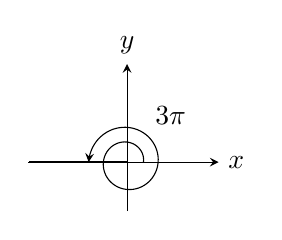
\begin{tikzpicture}
\begin{axis}[small,clip=false,axis equal,width=4cm,axis lines=middle,xlabel={$x$},xlabel style={at={(current axis.right of origin)},anchor=west},ylabel style={at={(current axis.above origin)},anchor=south},ylabel={$y$},xtick={\empty},ytick={\empty},ymin=-0.75,ymax=1.5]
\addplot[-stealth,domain=0:540,samples=100]({(0.25+0.25/400*x)*cos(x)},{(0.25+0.25/400*x)*sin(x)})node[pos=0.7,above right]{$3\pi$};
\draw[thick](axis cs:0,0)--(axis cs:-1.5,0);
\end{axis}
\end{tikzpicture}
\end{subfigure}%
\begin{subfigure}{0.25\textwidth}
\centering
\begin{tikzpicture}
\begin{axis}[small,clip=false,axis equal,width=4cm,axis lines=middle,xlabel={$x$},xlabel style={at={(current axis.right of origin)},anchor=west},ylabel style={at={(current axis.above origin)},anchor=south},ylabel={$y$},xtick={\empty},ytick={\empty},ymax=1]
\addplot[mark=none,thick] plot coordinates {(0,0) ({2*cos(-135)},{2*sin(-135)})};
\addplot[-stealth,domain=0:-135,samples=100]({(0.25-0.25/135*x)*cos(x)},{(0.25-0.25/135*x)*sin(x)})node[pos=0.7,below right]{$-\tfrac{3\pi}{4}$};
\end{axis}
\end{tikzpicture}
\end{subfigure}%
\begin{subfigure}{0.25\textwidth}
\centering
\begin{tikzpicture}
\begin{axis}[small,clip=false,axis equal,width=4cm,axis lines=middle,xlabel={$x$},xlabel style={at={(current axis.right of origin)},anchor=west},ylabel style={at={(current axis.above origin)},anchor=south},ylabel={$y$},xtick={\empty},ytick={\empty},ymax=1]
\addplot[-stealth,domain=0:-450,samples=100]({(0.25-0.25/450*x)*cos(x)},{(0.25-0.25/450*x)*sin(x)})node[pos=0.6,above right]{$-\tfrac{5\pi}{2}$};
\draw[thick](axis cs:0,0)--(axis cs:0,-1);
\end{axis}
\end{tikzpicture}
\end{subfigure}%
\caption{مثبت اور منفی ریڈیئن}
\label{شکل_ابتدا_زاویہ_ناپ}
\end{figure}

شکل \حوالہ{شکل_ابتدا_جسامت_اور_زاویہ} میں ایک جیسے اشکال کو دو مختلف ناپ میں دکھایا گیا ہے۔آپ دیکھ سکتے ہیں کہ جسامت بڑی یا چھوٹی کرنے سے زاویے تبدیل نہیں ہوتے ہیں۔یوں دونوں اشکال میں \عددی{\alpha+\beta=90^{\circ}} ہے۔ \عددی{x} اور \عددی{y} محدد پر اکائی فاصلہ کی ناپ کم اور زیادہ کرتے ہوئے اشکال کی جسامت تبدیل ہوتی ہے۔دونوں محدد پر اکائی فاصلہ ایک جیسا ہونا ضروری ہے۔آپ دیکھ سکتے ہیں کہ جسامت \عددی{k} گنا  کرنے سے تمام  سیدھی لمبائیاں \عددی{k} گنا ہوں گے۔کیا جسامت \عددی{k} گنا  کرنے سے لمبائی قوس بھی \عددی{k} گنا ہو گی؟ اس کا جواب ہے جی ہاں۔ آئیں اس حقیقت کا ثبوت دیکھیں۔
\begin{figure}
\centering
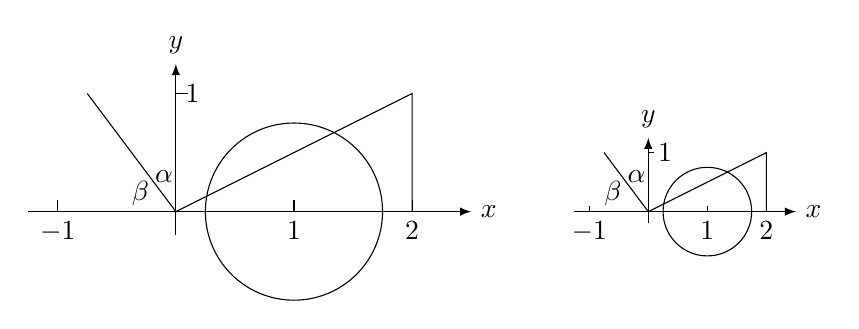
\begin{tikzpicture}[x=0.75cm,y=0.75cm]
\draw[-latex](-1.25,0)--(2.5,0)node[right]{$x$};
\draw[-latex](0,-0.2)--(0,1.25)node[above]{$y$};
\foreach \x in {-1,1,2} {\draw(\x,0)node[below]{$\x$}--++(0,0.1);}
\draw(0,1)node[right]{$1$}--++(0.1,0);
\draw(1,0) circle (0.75);
\draw(2,0)--(2,1)--(0,0);
\draw(0,0)--(-0.75,1);
\draw(-0.2,0.6)node[]{$\alpha$};
\draw(-0.6,0.3)node[]{$\beta$};
\begin{scope}[x={1.5cm},y={1.5cm},xshift={-6cm}]
\draw[-latex](-1.25,0)--(2.5,0)node[right]{$x$};
\draw[-latex](0,-0.2)--(0,1.25)node[above]{$y$};
\foreach \x in {-1,1,2} {\draw(\x,0)node[below]{$\x$}--++(0,0.1);}
\draw(0,1)node[right]{$1$}--++(0.1,0);
\draw(1,0) circle (0.75);
\draw(2,0)--(2,1)--(0,0);
\draw(0,0)--(-0.75,1);
\draw(-0.1,0.3)node[]{$\alpha$};
\draw(-0.3,0.15)node[]{$\beta$};
\end{scope}
\end{tikzpicture}
\caption{شکل بڑھانے یا گھٹانے کا زاویہ پر اثر نہیں پایا جاتا ہے۔}
\label{شکل_ابتدا_جسامت_اور_زاویہ}
\end{figure}

\begin{figure}
\centering
\begin{minipage}{0.45\textwidth}
\centering
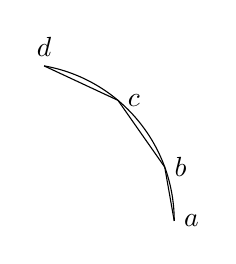
\begin{tikzpicture}
\draw([shift={(0:2)}]0,0) arc (0:80:2);
\coordinate (kA) at (0:2);
\coordinate (kB) at (20:2);
\coordinate (kC) at (50:2);
\coordinate (kD) at (80:2);
\draw(kA)node[right]{$a$}--(kB)node[right]{$b$}--(kC)node[right]{$c$}--(kD)node[above]{$d$};
\end{tikzpicture}
\caption{قوس کی لمبائی}
\label{شکل_ابتدا_قوس_لمبائی}
\end{minipage}\hfill
\begin{minipage}{0.45\textwidth}
\centering
\centering
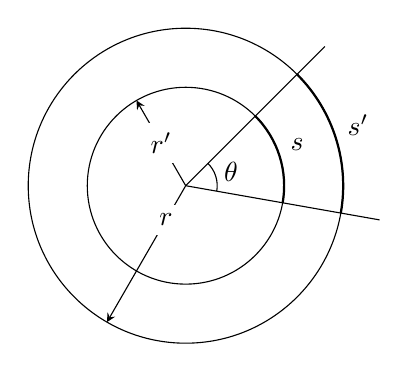
\begin{tikzpicture}
\draw(0,0) circle (1.25);
\draw(0,0) circle (2);
\draw(0,0)--++(-10:2.5);
\draw(0,0)--++(45:2.5);
\draw[thick]([shift={(-10:1.25)}]0,0) arc (-10:45:1.25);
\draw[thick]([shift={(-10:2)}]0,0) arc (-10:45:2);
\draw([shift={(-10:0.4)}]0,0) arc (-10:45:0.4);
\draw(17:0.6)node[]{$\theta$};
\draw(15:2)node[above right]{$s'$};
\draw(15:1.25)node[above right]{$s$};
\draw[-stealth](0,0)--++(120:1.25)node[pos=0.5,fill=white]{$r'$};
\draw[-stealth](0,0)--++(-120:2)node[pos=0.25,fill=white]{$r$};
\end{tikzpicture}
\caption{محیط دائرہ}
\label{شکل_ابتدا_دائرہ_اور_ریڈیئن}
\end{minipage}%
\end{figure}

شکل \حوالہ{شکل_ابتدا_قوس_لمبائی} میں قوس کی لمبائی جاننے کی خطر قوس پر مختلف نقطے منتخب کرتے ہوئے ان کے بیچ سیدھے خط کھینچے گئے ہیں۔ان سیدھے خطوط کی مجموعی لمبائی کو قوس کی تخمینی لمبائی لی جا سکتی ہے۔آپ دیکھ سکتے ہیں کہ قوس پر نقطوں کی تعداد بڑھا کر اس کو زیادہ ٹکڑوں میں تقسیم کرتے ہوئے قوس کی لمبائی اور سیدھے خطوط کی مجموعی لمبائی میں فرق کو ہم جتنا چاہیں کم کر سکتے ہیں۔اب اگر اس قوس کی جسامت کو \عددی{k} گنا کیا جائے تب ہر سیدھے خط کی لمبائی \عددی{k} گنا ہو گی لہٰذا ان کی مجموعی لمبائی (جو قوس کی لمبائی ہے) بھی \عددی{k} گنا ہو گی۔

شکل \حوالہ{شکل_ابتدا_دائرہ_اور_ریڈیئن} میں رداس \عددی{r} اور رداس \عددی{r'} کے دائرے دکھائے  گئے ہیں جہاں قوس \عددی{s} اور \عددی{s'} بھی دکھائے گئے ہیں۔چھوٹے دائرے کی جسامت بڑھاتے ہوئے بڑا دائرہ حاصل کیا جس سکتا ہے۔جسامت بڑھانے سے زاویے تبدیل نہیں ہوتے ہیں۔یوں دونوں دائروں کی رداس کا تناسب اور دکھائے گئے قوسین کا تناسب ایک جیسا ہو گا، یعنی:
\begin{align*}
\frac{s}{s'}=\frac{r}{r'}\quad \implies \quad s=r\frac{s'}{r'}
\end{align*}
اب اگر \عددی{r'=1} ہو تب ریڈیئن کی تعریف کی رو سے \عددی{\tfrac{s'}{r'}=\theta} ہو گا (جہاں زاویہ ریڈیئن میں ہو گا) لہٰذا درج بالا سے درج ذیل اہم ترین کلیہ حاصل ہوتا ہے۔
\begin{mdframed}[frametitle={قوس کی لمبائی اور ریڈیئن میں ناپے گئے زاویے کا تعلق}]
\begin{align*}
s=r\theta
\end{align*}
\end{mdframed}
% 
\begin{mdframed}[frametitle={زاویہ ناپنے کی روایت: ریڈیئن استعمال کریں}]
یہاں کے بعد اس کتاب میں زاویے کو ریڈیئن میں ناپا جائے گا۔جہاں زاویے کو ریڈیئن میں نہیں ناپا گیا ہو وہاں صریحاً بتلایا جائے گا۔یوں اگر ہم زاویہ \عددی{\tfrac{\pi}{6}} کی بات کریں تب اس سے مراد \عددی{\tfrac{\pi}{6}} ریڈیئن کا زاویہ ہو گا نا کہ \عددی{\tfrac{\pi}{6}} درجے کا زاویہ۔
\end{mdframed}

\ابتدا{مثال}
رداس \عددی{8} کے دائرے پر غور کریں۔ (الف) دائرے پر \عددی{2\pi} لمبائی کا قوس، دائرے کے مرکز پر کیا وسطی زاویہ بناتا ہے۔ (ب) اس قوس کی لمبائی تلاش کریں جو 
\عددی{\tfrac{3\pi}{4}} وسطی زاویہ بناتا ہو۔\\
حل:\quad
\begin{gather*}
\begin{aligned}
 s=r\theta=8(\tfrac{3\pi}{4})=6\pi \quad \text{(ب)}
\end{aligned}\quad\quad
\begin{aligned}
\theta=\frac{s}{r}=\frac{2\pi}{8}=\frac{\pi}{4} \quad \text{(الف)}
\end{aligned}
\end{gather*} 
\انتہا{مثال}
%================================

\جزوحصہء{چہ بنیادی تکونیاتی تفاعل}
آپ  زاویہ حادہ کے تکونیاتی تفاعل سے بخوبی واقف ہوں گے جو قائمہ مثلث کے اطراف کی لمبائیوں کی تناسب سے حاصل ہوتے ہیں (شکل \حوالہ{شکل_ابتدا_قائمہ_مثلث})۔ ہم انہیں تعریف کو وسعت دیتے ہوئے  زاویہ منفرجہ اور منفی زاویوں پر بھی لاگو کرتے ہیں جہاں معیاری مقام پر رداس \عددی{r} کے دائرے میں زاویہ پایا جاتا ہے۔ہم اب ان تکونیاتی تفاعل کو نقطہ \عددی{N(x,y)} کے محدد کی صورت میں بیان کرتے ہیں جہاں مبدا سے خارج ہوتا ہوا شعاع دائرے کو \عددی{N(x,y)} پر قطع کرتا ہے۔
\begin{figure}
\centering
\begin{minipage}[b][][b]{0.3\textwidth}
\centering
\begin{tikzpicture}
\path[name path=kX](0,0)--(3,0);
\draw(0,0)--++(30:2)coordinate(kA);
\draw(kA)--($(0,0)!(kA)!(3,0)$)coordinate(kB)--(0,0);
\RightAngle{(0,0)}{(kB)}{(kA)};
\draw[-stealth]([shift={(0:0.6)}]0,0) arc (0:30:0.6);
\draw(14:0.8)node[]{$\theta$};
\draw($(0,0)!0.5!(kB)$)node[below]{قاعدہ};
\draw($(kA)!0.5!(kB)$)node[right]{عمود};
\draw($(0,0)!0.5!(kA)$)node[above]{وتر};
\end{tikzpicture}
\end{minipage}\hfill
\begin{minipage}[b][][b]{0.66\textwidth}
\begin{gather*}
\begin{aligned}
\sin \theta&=\tfrac{\text{عمود}}{\text{وتر}},\\
\cos \theta&=\tfrac{\text{قاعدہ}}{\text{وتر}},\\
\tan \theta&=\tfrac{\text{عمود}}{\text{قاعدہ}},
\end{aligned}\quad
\begin{aligned}
\csc&=\tfrac{\text{وتر}}{\text{عمود}}\\
\sec&=\tfrac{\text{وتر}}{\text{قاعدہ}}\\
\cot&=\tfrac{\text{قاعدہ}}{\text{عمود}}
\end{aligned}
\end{gather*}
\end{minipage}%
\caption{قائمہ مثلث اور تکونیاتی تفاعل}
\label{شکل_ابتدا_قائمہ_مثلث}
\end{figure}

شکل \حوالہ{شکل_ابتدا_تفاعل_تکونیاتی} کو دیکھتے ہوئے ان تفاعل کو یہاں پیش کرتے ہیں۔
\begin{figure}
\centering
\begin{tikzpicture}
\draw[-latex](-1.5,0)--(2,0)node[right]{$x$};
\draw[-latex](0,-1.25)--(0,1.5)node[above]{$y$};
\draw(0,0)node[below left]{$M$} circle (1);
\draw[-latex](0,0)--++(135:1.7);
\draw[-stealth]([shift={(0:0.5)}]0,0) arc (0:135:0.5);
\draw(45:0.7)node[]{$\theta$};
\draw(135:1)node[circ]{}node[left]{$N(x,y)$};
\end{tikzpicture}
\caption{تکونیاتی تفاعل}
\label{شکل_ابتدا_تفاعل_تکونیاتی}
\end{figure}
